\begin{flushleft}
Lo script che abbimo implementato è il seguente:
\lstinputlisting[language=Matlab]{cap_4/es9/es9.m}
Nello script abbiamo prima definito le funzioni da studiare e creato un vettore rappresentante la costante $\epsilon$ in cui il primo elemento è il caso $\epsilon=0.1$ e il secondo è $\epsilon=0.2$ Dunque nei due cicli annidati vengono calcolati gli elementi delle matrici $y_{i,1}$ e $y_{i,2}$ in cui nella prima colonna si hanno i valori della prima funzione con $\epsilon_1$ e nella seconda con $\epsilon_2$ (il valore di $\gamma_i$ varia per ogni iterazione del ciclo in modo aleatorio). I quali vengono dati in input alla nostra funzione polBetter per effettuare i test richiesti, da cui si ricavano i coefficienti. Alla fine i risultati stampati sono:
\begin{figure}[H]
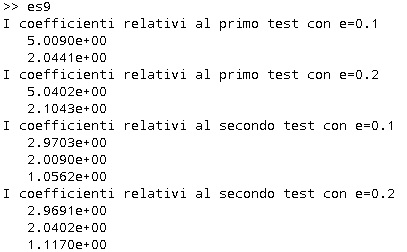
\includegraphics[left, width=400px, height=200px]{cap_4/es9/es49.png}
\end{figure}
\end{flushleft}